\documentclass[../DS06.tex]{subfiles}
\graphicspath{{./figures/}}

% \subimport{/home/nora/Documents/Enseignement/Prepa/bpep/exercices/DS/HP_electrostatique/}{sujet.tex}

\begin{document}

\prblm[45]{Le haut-parleur électrostatique\ifcorrige{~\small\textit{(D'après
			Centrale 2013 TSI)}}}

\enonce{
	\noindent
	\begin{isd}
		Deux disques conducteurs de même rayon, parallèles, sont écartés d'une
		faible distance $e$. L'un d'eux est fixe (la base), l'autre
		constituant la membrane est mobile en translation selon l'axe $Oz$.
		\bigbreak
		La membrane de surface $S$ est rappelée vers la position $z = 0$ par la
		force de rappel élastique $\Ff_r = -kz\uz$ (on considère donc $\ell_0 = 0$).
		L'air séparant les disques est assimilable, du point de vue électrostatique,
		au vide.
		\bigbreak
		Lorsqu'on établit une différence de potentiel $U$ entre les disques, il
		apparait une charge électrique $Q$ sur la base et une charge opposée $-Q$
		sur la membrane. Ces charges sont réparties uniformément sur chaque disque.
		On négligera l'effet du poids.
		\tcblower
		\begin{center}
			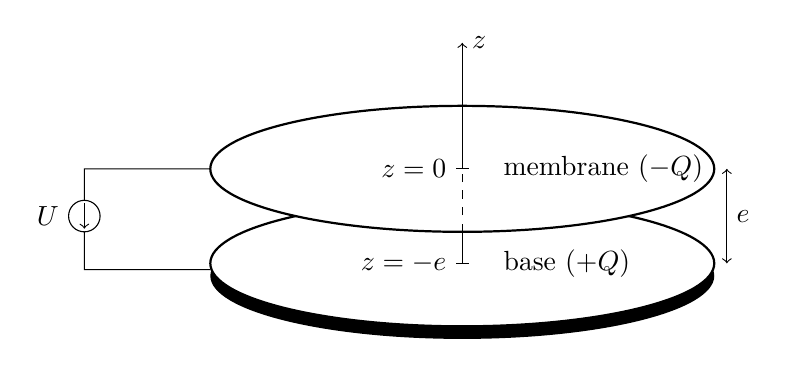
\begin{tikzpicture}[scale=.8]
				\fill (0,-0.2) ellipse [x radius=4,y radius=1];
				\draw [thick,fill=white] (0,0) ellipse [x radius=4,y radius=1];
				\draw [thin] (0,0) -- +(0,2);
				\draw [thick,fill=white] (0,1.5) ellipse [x radius=4,y radius=1];
				\draw [thin,dashed] (0,0.5) -- (0,1.5);
				\draw [thin,->] (0,1.5) -- +(0,2) node [right] {$z$};
				\draw [thin] (0.1,1.5) -- (-0.1,1.5) node [left] {$z=0$};
				\draw [thin] (0.1,0) -- (-0.1,0) node [left] {$z=-e$};
				\draw [<->] (4.2,0) -- node [auto,swap] {$e$} +(0,1.5);
				\draw (-4,1.5) -| (-6,1) (-6,0.75) circle [radius=0.25] (-6,0.5) |- (-4,-0.1);
				\draw [->] (-6,0.95) -- (-6,0.55);
				\node at (-6.25,0.75) [left] {$U$};
				\node at (.5,0) [right] {base ($+Q$)};
				\node at (.5,1.5) [right] {membrane ($-Q$)};
			\end{tikzpicture}
			\captionof{figure}{Schéma du dispositif.}
		\end{center}
	\end{isd}
}

\subsection{Force exercée sur la membrane}

\enonce{
	La base étant assimilable à un plan infini, la charge portée par la base crée
	un champ électrique
	\[
		\Ef = \frac{Q}{2S\ep_0}\uz\quad \mbox{pour}\quad z>-e
	\]
	On peut montrer que la capacité du condensateur s'écrit
	$C = \frac{S\ep_0}{e+z}$. Ainsi la capacité évolue en fonction de la distance
	$(e+z)$ séparant les deux armatures.
}

\QR[2]{%
	Rappeler la relation liant la tension $U$, la capacité $C$ et la charge $Q$
	portée par les armatures d'un condensateur. En déduire l'expression de la
	charge $Q$ en fonction de $z$, $U$ et des constantes du problème.
}{%
	\[
		Q \stm[-1]{=} CU \qqdc \boxed{Q \stm[-1]{=} \frac{US\ep_0}{e+z}}
	\]
}

\QR[3]{%
	Déterminer la force électrique $\Ff_e$ subie par la membrane.
	Est-elle attractive ou répulsive~?
}{%
	\[
		\Ff_e \stm{=} -Q\Ef = -\frac{Q^2}{2S\ep_0}\uz
		\Lra
		\boxed{\Ff \stm{=} -\frac{S\ep_0U^2}{2(e+z)^2}\uz}
	\]
	La force est attractive \pt{1} car orientée selon $-\uz$.
}

\subsection{Étude énergétique}

\QR[2]{%
	Définir ce qu'est une force conservative et son lien avec l'énergie
	potentielle associée.
}{%
	Une force est dite conservative si \textbf{son travail ne dépend pas du chemin suivi} \pt{1}, c'est-à-dire qu'elle dérive d'une énergie potentielle~:
	\[
		\boxed{\delta W(\Ff_e) \stm[-1]{=} -\dd{\Ec_p}}
	\]
}

\QR[6]{%
	Établir l'expression de l'énergie potentielle $\Ec_{p,e}(z)$ électrique. On
	prendra son origine en $z = 0$.
}{%
	On calcule le travail élémentaire $\delta W(\Ff_e) \stm[-1]{=} \Ff_e\cdot
		\dd\OM$, avec $d\OM \stm[-1]{=} \dd{x}\vv{u_x}+\dd{y}\vv{u_y}+\dd{z}\uz$~:
	\begin{gather*}
		\delta W(\Ff_e) =
		-\frac{S\ep_0U^2}{2(e+z)^2}\dd{z} \stm[-1]{=}
		-\dd\left ( -\frac{S\ep_0U^2}{2(e+z)} \right ) =
		-\dd{\Ec_{p,e}}
		\\\Lra
		\Ec_{p,e}(z) \stm[-1]{=}
		-\frac{S\ep_0U^2}{2(e+z)} + \underbracket[1pt]{A}_{=\cte}
		\qor
		\Ec_{p,e}(0) = 0
		\Ra
		A \stm[-1]{=} \frac{S\ep_0U^2}{2e}
		\\\Lra
		\boxed{
			\Ec_{p,e}(z) \stm[-1]{=}
			-\frac{S\ep_0U^2}{2}\left ( \frac{1}{e+z} -\frac{1}{e}\right )
		}
	\end{gather*}
}

\QR[3]{%
	L'énergie mécanique de la membrane est-elle conservée~?
}{%
	La membrane, étudiée dans le référentiel du laboratoire supposé galiléen, est
	soumise~:
	\begin{itemize}
		\litem{10pt}{\pt{1}} à la force de rappel élastique qui est une force
		conservative,
		\litem{10pt}{\pt{1}} à la force électrique qui est une force conservative.
	\end{itemize}
	Donc le système est conservatif \pt{1}.
}

\QR[2]{%
	Exprimer l'énergie potentielle totale du système $\Ec_p(z)$. On rappelle que
	l'origine de l'énergie potentielle est prise en $z = 0$.
}{%

	C'est la somme \pt{1} de l'énergie potentielle élastique $\Ec_{p,\rm el}$ et de
	l'énergie potentielle électrique. Comme l'énergie potentielle est nulle en $z
		= 0$, on en déduit que la constante de $\Ec_{p, \rm el}$ est nulle, et ainsi~:
	\[
		\boxed{
			\Ec_p(z) \stm{=}
			\frac{1}{2}{kz^2}-
			\frac{S\ep_0U^2}{2}\left( \frac{1}{e+z} -\frac{1}{e}\right)
		}
	\]
}

\QR[3]{%
	Expliquer en quoi l'étude de $\Ec_p(z)$ permet de prévoir l'ensemble des
	valeurs possibles de $z$.
}{%
	Le système est un système conservatif à un degré de liberté, donc $\Ec_m
		\stm[-1]{=} \Ec_c(z)+\Ec_p(z) \stm[-1]{=} \cte$. Or $\Ec_c\geq 0$, d'où les
	valeurs possibles de $z$ vérifient
	\[
		\boxed{\Ec_p(z) \stm[-1]{\leq} \Ec_m}
	\]
}

\QR[3]{%
	Montrer que les positions d'équilibre possibles $z_0$ vérifient $z_0(e+z_0)^2
		= A$. Donner l'expression de $A$.
}{%
	Les positions d'équilibre $z_0$ vérifient
	\[
		\dv{\Ec_p}{z}\/(z_0) \stm[-1]{=} 0
		\Lra
		kz_0+\frac{S\ep_0 U^2}{2(e+z_0)^2} = 0
		\Lra
		\boxed{z_0(e+z_0)^2 \stm[-1]{=} -\frac{S\ep_0}{2k}U^2}
		\qav
		\boxed{A \stm[-1]{=} -\frac{S\ep_0}{2k}U^2}
	\]
}

\QR[6]{\label{Q:z0}
	On étudie la fonction $f(z) = z(e+z)^2$ pour $z\in[-e,0]$. Montrer qu'elle
	admet un minimum une valeur $z_m$ à déterminer. Préciser la valeur de $f$ en
	ce minimum. En déduire la valeur maximale $U_m$ de $U$ pour qu'il y ait deux
	positions d'équilibre $z_1$ et $z_2$ telles que $-e < z_1 < z_2 < 0$.
}{%
	\smallbreak
	\vspace{-30pt}
	\noindent
	\begin{minipage}[c]{.45\linewidth}
		Valeurs extrêmes~:
		\begin{itemize}
			\item $f(-e) = 0$
			\item $f(0) = 0$
		\end{itemize}
		Étude de la dérivée~:
		\begin{itemize}
			\item $f'(z) = (e+z)^2+2z(e+z) \stm[-1]{=} (e+z)(3z+e)$
			\item $f'(z) = 0$ si $z = -e$ ou $z = -e/3$ \pt{1}
			\item en $z = -e$~: maximum local de $f(z)$
			\item en $z = -e/3$~: minimum de $f(z)$ \pt{1}
		\end{itemize}
	\end{minipage}
	\hfill
	\begin{minipage}[c]{.45\linewidth}
		~
		\begin{center}
			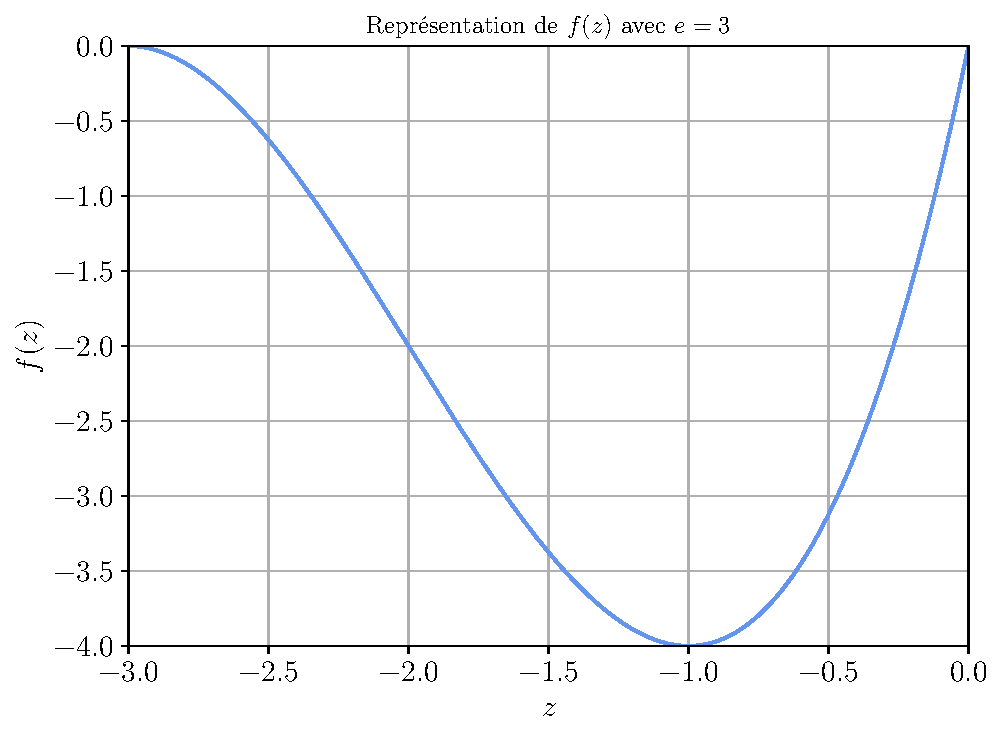
\includegraphics[width=\linewidth]{fz}
			\captionof{figure}{Représentation de $f(z)$.}
			\label{fig:fz}
		\end{center}
	\end{minipage}
	\smallbreak
	La fonction $f$ admet un minimum en $\boxed{z_m = -e/3}$, alors $\boxed{f(z_m)
			\stm[-1]{=} -4e^3/27}$.
	\smallbreak
	On en déduit que pour $z\in[-e,0]$, $f(z)\in[-4e^3/27,0]$. Il faut donc que
	$A\in [-4e^3/27,0]$~:
	\[
		-4e^3/27 \stm[-1]{\leq} -\frac{S\ep_0}{2k}U^2\leq 0
		\qdc
		\boxed{U \stm[-1]{\leq} \sqrt{\frac{8ke^3}{27\ep_0S}} = U_m}
	\]
}

\QR[1]{%
	Que valent $z_1$ et $z_2$ pour $U = U_m$~?
}{%
	D'après la réponse à la question précédente, $\boxed{z_1 \stm[-1]{=} z_2 =
			-e/3}$.
}

\QR[4]{\label{Q:stab}
	Montrer que la position d'équilibre stable vérifie $z_0>-e/3$.
}{%
	On étudie le signe de la dérivée seconde de l'énergie potentielle en $z_0$~:
	\[
		\dv[2]{\Ec_p}{z} \stm[-1]{=}
		k-\frac{S\ep_0U^2}{(e+z)^3} =
		k\left(1- \frac{S\ep_0U^2}{k(e+z)^3}\right)
	\]
	Or la position d'équilibre vérifie $\frac{S\ep_0U^2}{k} = -2z_0(e+z_0)^2$, donc
	\[
		\dv[2]{\Ec_p}{z}\/(z_0) \stm[-1]{=} k\left (1+\frac{2z_0}{e+z_0} \right )
	\]
	Si la position d'équilibre $z_0$ est stable, alors $\dv[2]{\Ec_p}{z}\/(z_0)
		\stm[-1]{>} 0$, soit
	\[
		1+\frac{2z_0}{e+z_0}>0
		\quad \Leftrightarrow \quad
		\boxed{z_0 \stm[-1]{>} -e/3}
	\]
}

\QR[3]{%
	{\em Application numérique}. On prend $z_0 = -e / 100$ pour la position d'équilibre stable,
	$e = \SI{3}{\milli\meter}$, $S = \SI{0,05}{\meter^2}$, $k = \SI{1000}{\newton\cdot \meter^{-1}}$ et
	$\ep_0 = \SI{8.85e-12}{\farad\cdot \meter^{-1}}$. Déterminer $U$ et $U_m$.
}{%
	\vspace{-15pt}
	\[
		\boxed{U \stm[-1]{=} \sqrt{-z_0(e+z_0)^2\cdot \frac{2k}{S\ep_0}}}
		\Lra
		\xul{U \stm[-1]{=} \SI{1,1}{\kilo\volt}}
		\qqet
		U_m = \sqrt{\frac{8ke^3}{27\ep_0S}}
		\Lra
		\xul{U_m \stm[-1]{=} \SI{4,3}{\kilo\volt}}
	\]
}

% \subsection{Portrait de phase}
%
% \enonce{
% La figure \ref{fig:portrait} correspond au portrait de phase tracé pour $U = U_0$.
%
% \begin{minipage}{0.5\linewidth}
% \figCapRaw{portraitU0}{Portrait de phase pour $U = U_0$\label{fig:portrait}}
% \end{minipage}
% \begin{minipage}{0.5\linewidth}
% \figCapRaw{z-U0}{Évolution temporelle de $z/e$ pour $U = U_0$, avec différentes conditions initiales.\label{fig:z}}
% \end{minipage}
% }
%
% \QR{%
% Préciser le sens de parcours des trajectoires de phase. Justifier votre réponse.
% }{%
% Les trajectoires de phase sont orientées de gauche à droite dans le demi-plan supérieur car $\dot z>0$, donc $z(t)$ est une fonction croissante, 
% et de droite à gauche dans le demi-plan inférieur.
% }
%
% \QR{%
% Dénombrer les positions d'équilibre. Préciser leur stabilité. Est-ce en accord avec vos réponses aux questions
% \ref{Q:z0} et \ref{Q:stab}.
% }{%
% On constate deux positions d'équilibre, ce qui est cohérent car $U_0<U_m$.
%
% La position d'équilibre stable est proche de $0$. Ce qui est normal car pour $U = U_0$, $z_1 = -0,01e$. On a bien que $z_1>-e/3$.
%
% La position d'équilibre instable est $z_2\approx -0,9e$.
% }
% \enonce{
% La figure \ref{fig:z} présente l'évolution temporelle de $z/e$ pour différentes conditions initiales.
% }
%
% \QR{%
% Peut-on dire qu'il y a isochronisme des oscillations~? On définira ce terme.
% }{%
% On parle d'isochronisme des oscillations quand la période des oscillations d'un système est indépendante des conditions initiales. 
% Ce n'est pas le cas ici.
% }

\subsection{Dynamique}

\enonce{
	On étudie les petits mouvements de la membrane au voisinage de la position
	d'équilibre stable $z_0 = -e/100$ et on pose $z(t) = z_0 + \xi(t)$ avec
	$\abs{\xi(t)} \ll e + z_0$.
}

\QR[4]{%
	Écrire l'équation différentielle vérifiée par $\xi(t)$. Définir la pulsation propre en fonction de $k$, $m$, $e$ et $z_0$.
}{%
	On applique la loi de la quantité de mouvement à la membrane, projetée selon
	$\uz$~: $m\dv[2]{z}{t} = F(z) = -\dv{\Ec_p}{z}$, (ou la conservation de
	l'énergie mécanique).

	On effectue un développement limité \pt{1} autour de $z_0$~: $m\dv[2]{z}{t} =
		-\dv{\Ec_p}{z}\/(z_0)-(z-z_0)\dv[2]{\Ec_p}{z}\/(z_0)$

	\begin{isd}
		\begin{align*}
			\beforetext{Or $\ddot z \stm[-1]{=}\ddot\xi$, donc}
			\dv[2]{\xi}{t}+\frac{1}{m}\dv[2]{\Ec_p}{z}\/(z_0)\xi & =
			0
			\\\Lra
			\Aboxed{
				\dv[2]{\xi}{t} +
			\frac{k}{m}\left(1+\frac{2z_0}{e+z_0}\right)\xi      & \stm[-1]{=} 0
			}
		\end{align*}
		\tcblower
		On pose donc la pulsation propre
		\begin{gather*}
			\boxed{
				\omega_0 \stm[-1]{=}
				\sqrt{\frac{k}{m}\left(1+ \frac{2z_0}{e+z_0} \right)}
			}
		\end{gather*}
	\end{isd}
}

\QR[3]{%
	La membrane est une feuille d'aluminium d'épaisseur $a = \SI{20}{mm}$, d'aire
	$S = \SI{0.05}{m^{2}}$ et de masse volumique $\rho =\SI{2.7e3}{kg.m^{-3}}$.
	Calculer la période propre $T_0$ du système.
}{%
	\begin{isd}
		\begin{align*}
			\w_0 & \stm[-1]{=} \frac{2\pi}{T_0}
			\\\Lra
			T_0  & = 2\pi \sqrt{\frac{m}{k}\left( \frac{e+z_0}{e+3z_0} \right)}
			\\\Lra
			\Aboxed{
			T_0  & \stm{=}
				2\pi \sqrt{\frac{\rho aS}{k}\left( \frac{e+z_0}{e+3z_0} \right)}
			}
		\end{align*}
		\tcblower
		\begin{gather*}
			\Lra
			\xul{T_0 \stm{=} \SI{10.4}{ms}}
			\qav
			\left\{
			\begin{array}{rcl}
				\rho & = & \SI{2.7e3}{kg.m^{-3}}
				\\
				a    & = & \SI{20e-6}{m}
				\\
				S    & = & \SI{5e-2}{m^{2}}
				\\
				k    & = & \SI{1000}{N.m^{-1}}
				\\
				e    & = & \SI{3e-3}{m}
				\\
				z_0  & = & -\frac{e}{100} = \SI{-3e-5}{m}
			\end{array}
			\right.
		\end{gather*}
	\end{isd}


}
\end{document}
